% Graphical Abstract for EmergentHoney
% 描述：用于 Elsevier 投稿的图形摘要
%
% 布局设计 (左→右叙事流):
%
% ┌─────────────────────────────────────────────────────────────────────┐
% │                                                                     │
% │  [Ant Colony]  ──→  [Pheromone Engine]  ──→  [Self-Organizing      │
% │  Inspiration        τ_{ij} update           Honeypot Swarm]        │
% │                                                                     │
% │       ↓                    ↓                       ↓                │
% │  Biological         Attack Pheromone       LLM Phenotype           │
% │  Isomorphism        τ(t+1)=(1-ρ)τ+Δτ      Generation              │
% │                                                                     │
% │                    [Network Topology]                               │
% │                    with deployed honeypots                          │
% │                    (proliferate/migrate/mutate)                     │
% │                                                                     │
% │  Key Results:                                                       │
% │  ✓ ADT: 247.3s (2.3× baseline)                                    │
% │  ✓ DEI > 1 (emergence proved)                                      │
% │  ✓ 76% prediction accuracy                                         │
% │                                                                     │
% └─────────────────────────────────────────────────────────────────────┘
%
% 实际图形建议使用 Adobe Illustrator / Figma 制作高分辨率版本
% 以下为 TikZ 原型

\documentclass[border=5mm]{standalone}
\usepackage{tikz}
\usetikzlibrary{arrows.meta, positioning, shapes, fit, backgrounds, calc}
\usepackage{amsmath}

\begin{document}
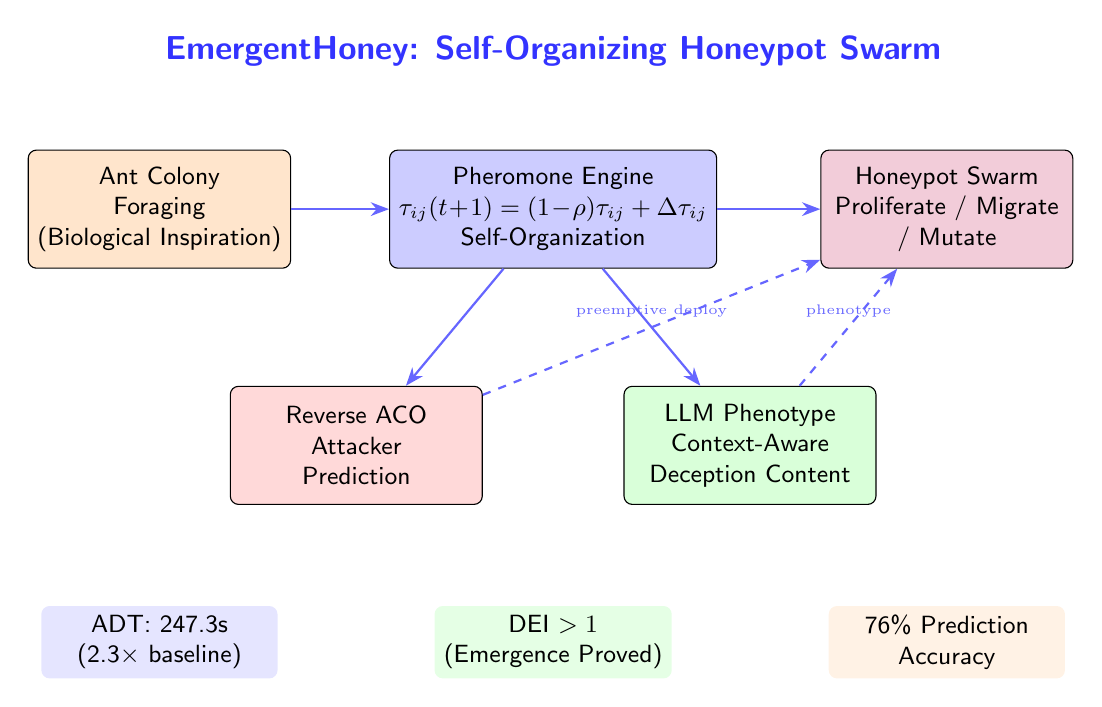
\begin{tikzpicture}[
    >=Stealth,
    box/.style={draw, rounded corners=3pt, minimum width=3.2cm, minimum height=1.5cm,
                align=center, font=\small\sffamily},
    result/.style={draw=none, fill=green!10, rounded corners=3pt, minimum width=3cm,
                   minimum height=0.8cm, align=center, font=\small\sffamily},
    arrow/.style={->, thick, color=blue!60},
]

% 第一层：灵感 → 核心 → 输出
\node[box, fill=orange!20] (bio) at (0,0)
    {Ant Colony\\Foraging\\(Biological Inspiration)};

\node[box, fill=blue!20] (engine) at (5,0)
    {Pheromone Engine\\$\tau_{ij}(t\!+\!1) = (1\!-\!\rho)\tau_{ij} + \Delta\tau_{ij}$\\Self-Organization};

\node[box, fill=purple!20] (swarm) at (10,0)
    {Honeypot Swarm\\Proliferate / Migrate\\/ Mutate};

% 第二层
\node[box, fill=red!15] (reverse) at (2.5,-3)
    {Reverse ACO\\Attacker\\Prediction};

\node[box, fill=green!15] (llm) at (7.5,-3)
    {LLM Phenotype\\Context-Aware\\Deception Content};

% 箭头
\draw[arrow] (bio) -- (engine);
\draw[arrow] (engine) -- (swarm);
\draw[arrow] (engine) -- (reverse);
\draw[arrow] (engine) -- (llm);
\draw[arrow, dashed] (reverse) -- (swarm) node[midway, above, font=\tiny] {preemptive deploy};
\draw[arrow, dashed] (llm) -- (swarm) node[midway, above, font=\tiny] {phenotype};

% 结果
\node[result, fill=blue!10] at (0,-5.5) {ADT: 247.3s\\(2.3$\times$ baseline)};
\node[result, fill=green!10] at (5,-5.5) {DEI $> 1$\\(Emergence Proved)};
\node[result, fill=orange!10] at (10,-5.5) {76\% Prediction\\Accuracy};

% 标题
\node[font=\large\bfseries\sffamily, color=blue!80] at (5,2)
    {EmergentHoney: Self-Organizing Honeypot Swarm};

\end{tikzpicture}
\end{document}
